\documentclass[tikz, preview]{standalone}

\usepackage{amsfonts, amsthm, amssymb, amsmath, stmaryrd, etoolbox}
\usepackage{tikz}
\usepackage[all,2cell]{xy}
\usetikzlibrary{matrix,arrows,shapes,decorations.markings,decorations.pathreplacing}
\definecolor{rewritecolor}{rgb}{0,.9,1}
\tikzset{rewritenode/.style={shape=circle,fill=rewritecolor,scale=0.25,font=\Huge}}
\tikzset{RWopen/.style={shape=circle,draw=black,fill=white,scale=0.5,font=\Huge}}
\tikzset{RWclosed/.style={shape=circle,fill=black,scale=0.5,font=\Huge}}
\tikzset{CDnode/.style={shape=circle,fill=white,scale=.5}}
\tikzset{zxgreen/.style={shape=circle,draw,thick,fill=green}}
\tikzset{zxred/.style={shape=circle,draw,thick,fill=red}}
\tikzset{zxyellow/.style={shape=rectangle,draw,thick,fill=yellow}}
\tikzset{zxdiamond/.style={shape=diamond,fill=black,inner sep=2.75}}
\tikzset{zxopen/.style={shape=circle,draw,thick,inner sep=2pt}}
\tikzset{->-/.style={decoration={markings,mark=at position .5 with {\arrow{>}}},postaction={decorate}}}

\begin{document}
\[
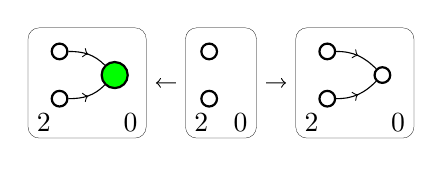
\begin{tikzpicture}
\begin{scope}[shift={(-0.8,0.1)}]
\node [zxgreen,label={}] (v1) at (1,-0.4) {};
\node [zxopen] (v2) at (0.3,-0.1) {};
\node [zxopen] (v3) at (0.3,-0.7) {};
%
\draw [->-] (v2) to [in=135,out=0] (v1);
\draw [->-] (v3) to [in=-135,out=0] (v1);
%
\node at (0.1,-1) {$2$};
\node at (1.2,-1) {$0$};
\node (v11) at (1.4,-0.5) {};
\draw [ultra thin, rounded corners] (-0.1,0.2) rectangle (1.4,-1.2);
\end{scope}
%
%
%
\begin{scope}[shift={(4.1,-0.1)}]
\node [zxopen] (v1) at (-2.7,0.1) {};
\node [zxopen] (v3) at (-2.7,-0.5) {};
\draw [ultra thin, rounded corners] (-3,0.4) rectangle (-2.1,-1);
\node at (-2.8,-0.8) {$2$};
\node at (-2.3,-0.8) {$0$};
\node (v12) at (-3,-0.3) {};
\node (v14) at (-2.1,-0.3) {};
\end{scope}
%
%
%
\begin{scope}[shift={(4.5,-0.5)}]
\node [zxopen] (v1) at (-0.9,0.2) {};
\node [zxopen] (v2) at (-1.6,0.5) {};
\node [zxopen] (v3) at (-1.6,-0.1) {};
%
\draw [->-] (v2) to [in=135,out=0] (v1);
\draw [->-] (v3) to [in=-135,out=0] (v1);
%
\node at (-1.8,-0.4) {$2$};
\node at (-0.7,-0.4) {$0$};
\draw [ultra thin, rounded corners] (-2,0.8) rectangle (-0.5,-0.6);
\node (v13) at (-2,0.1) {};
\end{scope}
%
%
%
\draw [<-] (v11) edge (v12);
\draw [<-] (v13) edge (v14);
\end{tikzpicture}
\]
\end{document}
